\documentclass[tikz]{standalone}
\usepackage[utf8]{inputenc}
\usetikzlibrary{intersections}

\definecolor{DarkBlue}{rgb}{0.0,0.0,0.6}
\definecolor{DarkRed}{rgb}{0.7,0.2,0.2}

\begin{document}

% hyperbola addition
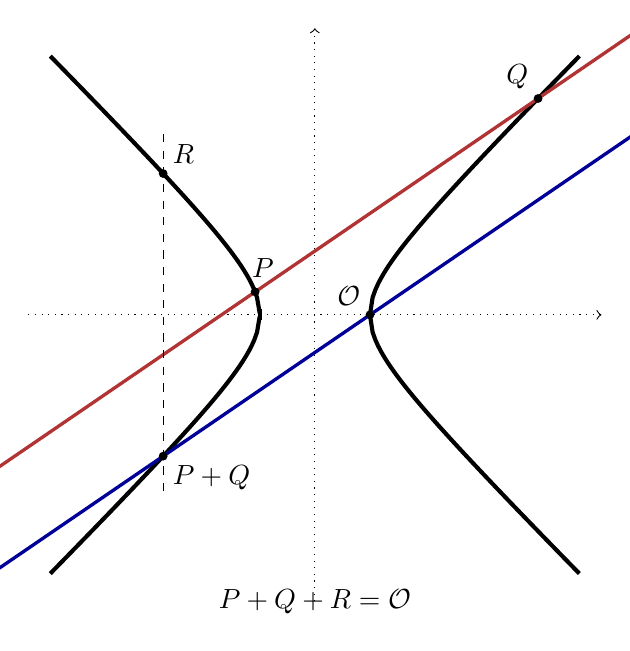
\begin{tikzpicture}[scale=.7]
\def\ptsize{.08}
\draw[->,dotted] (-5.2, 0) -- (5.2,0);
\draw[->,dotted] (0,-5.2) -- (0,5.2);
\coordinate (inf) at (1,0);
\path[draw,name path=leftup,samples=80,line width=1.5pt,domain=-4.8:-1] plot (\x, {sqrt((\x)^2 - 1)});
\draw[line width=1.5pt] (-1,-.1) -- (-1,.1);
\path[draw,name path=leftdown,samples=80,line width=1.5pt,domain=-4.8:-1] plot (\x, {-sqrt((\x)^2 - 1)});
\path[draw,name path=rightup,samples=80,line width=1.5pt,domain=1:4.8] plot (\x, {sqrt((\x)^2 - 1)});
\path[draw,name path=rightdown,samples=80,line width=1.5pt,domain=1:4.8] plot (\x, {-sqrt((\x)^2 - 1)});

\coordinate (P) at (-1.083,.417);
\node[shift={(.1,.3)}] at (P) {$P$};
\coordinate[label=above left:$Q$] (Q) at (4.05,3.925);
\coordinate[label=above right:$R$] (R) at (-2.752,2.564);
\coordinate[label=below right:$P+Q$] (S) at (-2.752,-2.564);

\draw[DarkRed,shorten >= -5cm,shorten <= -5cm,line width=1.2pt] (P) -- (Q);
\draw[DarkBlue,shorten >= -5cm,shorten <= -5cm,line width=1.2pt] (inf) -- (S);
\draw[dashed,shorten >= -.5cm,shorten <= -.5cm] (R) -- (S);

\fill (inf) circle (\ptsize);
\fill (P) circle (\ptsize);
\fill (Q) circle (\ptsize);
\fill (R) circle (\ptsize);
\fill (S) circle (\ptsize);
\node[above left] at (inf) {$\mathcal{O}$};
\node at (0,-5.2) {$P+Q+R=\mathcal{O}$};

\end{tikzpicture}

\end{document}